\documentclass[11pt]{article}

\usepackage[T1]{fontenc} % extended font encoding
\usepackage{enumerate} % lists
\renewcommand{\familydefault}{\sfdefault} % sans-serif
\usepackage{microtype} % better text justification
\usepackage{graphicx} % allow including pictures
\usepackage{color} % colors for pictures
\usepackage{textcomp} % for textminus
\usepackage{pagecolor} % background color for the first page
\usepackage{afterpage} % ditto ^^
\usepackage{tikz} % flow graph
\usetikzlibrary{dsp,chains}
\usepackage{parskip} % vertical paragraph spacing
\usepackage{hyperref} % links
\usepackage[a4paper, landscape, margin=1.5cm]{geometry} % basic geometry
\fboxsep=5mm % minibox spacing
\pagenumbering{gobble} % disable page numbering
\renewcommand{\thefootnote}{\arabic{footnote}} % use numbers for footnotes
\renewcommand{\thempfootnote}{\arabic{mpfootnote}} % ditto for minipages

% Style for a simple numbered list
\newenvironment{packed_enumerate}{
\begin{enumerate}
  \setlength{\itemsep}{1pt}
  \setlength{\parskip}{0pt}
  \setlength{\parsep}{0pt}
}{\end{enumerate}}

% Style for a roman literal numbered list
\newenvironment{packed_enumerate_i}{
\begin{enumerate}[I]
  \setlength{\itemsep}{1pt}
  \setlength{\parskip}{0pt}
  \setlength{\parsep}{0pt}
}{\end{enumerate}}


% Metadata
\pdfinfo{
   /Author (Zlosynth Instruments)
   /Title  (Kaseta - User Manual)
}

\begin{document}

% Front page should be black
\pagecolor{black}\afterpage{\nopagecolor}

% Front title
\title{\textcolor{white}{MANUAL}}
\author{}
\date{}

% Left column of the front page
\begin{minipage}{0.4\textwidth}
\color{white}
\maketitle

% Overview box
\noindent\colorbox{white}
{
\begin{minipage}{0.85\textwidth}\color{black}
Kaseta is a multi-purpose module inspired by reel-to-reel tape machines. It
simulates magnetic hysteresis to provide warm saturation, its four independent
delay lines can be used to sculpt rhythms or feedback loops, and it offers wow
and flutter control. The module also goes beyond typical tape machine features,
with free-moving delays, trigger sequencing, and an internal oscillator.
\end{minipage}
}

\vspace{1cm}

% Specs table
\begin{minipage}{0.8\textwidth}\color{white}
\begin{tabular}{@{}rl@{}}
  Width & 20 HP \\
  Depth & 28 mm \\
  % TODO: Needs to be re-measured
  Power & +12 V (85 mA), \textminus12 V (7 mA) \\
  Input impedance & 100 kΩ \\
  CV inputs & \textminus5 to +5 V, 16-bit, 1 kHz \\
  Trigger output & 0 to +5 V, 10 ms \\
  Audio & 24-bit, 48 kHz
\end{tabular}
\end{minipage}

\vspace{1cm}

% Features list
\begin{minipage}{0.8\textwidth}\color{white}
\begin{tabular}{@{}l}
  - Delay with 4 reading heads \\
  - Up to 5 minutes of audio recording \\
  - Tape saturation simulation \\
  - Wow and flutter effects \\
  - Tone control \\
  - Voltage-controlled oscillator \\
  - Trigger sequencer \\
  - Stereo output
\end{tabular}
\end{minipage}

\end{minipage}%
% Right column
\begin{minipage}{0.6\textwidth}
\vspace{8mm}

% Illustration of the panel
\begin{center}
  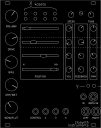
\includegraphics[width=0.8\textwidth]{schema.pdf}
\end{center}

\end{minipage}

% Start of the quick start page
\newpage
\color{black}

% Left column
\begin{minipage}[t]{0.45\textwidth}
\setlength{\parskip}{6pt}

\section{Installation}

Kaseta is 20 HP wide. It is powered by a +12V/{\textminus}12V 2\texttimes5
connector. The red stripe (\textminus12V) has to be connected on the side of the
board marked with the white line. The module must be mounted in a eurorack case.

\vspace{1cm}

\section{Controls, inputs and outputs}

There is one AC coupled audio input IN, and two stereo outputs LEFT and RIGHT.
They all operate in the range from \textminus5 to +5 V.

There is a total of 23 knobs. With the four identical rows (H) controlling four
independent delay reading heads.

The button (B) serves for tempo tap-in and access to secondary attributes of
some knobs:
Position of a filter set through TONE,
unlimited hysteresis enabled through DRIVE,
and internal oscillator enabled through PRE-AMP.

The four CONTROL inputs accept voltage from \textminus5 to +5 V and can be
mapped to any of the knobs. Values set by the knob and the control input are
summed together.

For most attributes, summing the minimal value of the knob with +5 V control
input would produce the maximum value of the attribute. 0 V on the control input
would not affect the attribute, and \textminus5 with maximum value on the knob
would lead to the minimum value of the attribute.

For TONE and WOW/FLUT, the maximum control input would only offset the
value to its middle point.

For the internal oscillator, the control input follows the 1V/oct standard, with
the knob adding an offset of \textminus2 to +2 octaves.

The display (X) visualizes dialed-in attributes, warnings and configuration.

The LED (Y) and IMPULSE output are triggered at intervals controlled by the
delay heads.

\end{minipage}%
\begin{minipage}{0.05\textwidth}
\phantom{ }
\end{minipage}%
% Right column
\begin{minipage}[t]{0.45\textwidth}
\setlength{\parskip}{6pt}

\section{Mapping}

Each of the four multi-purpose control inputs can be mapped to any of the knobs:

\begin{packed_enumerate}
  \item Plug a cable into one of the control inputs.
  \item Display will signalize mapping.
  \item Turn the desired target knob.
\end{packed_enumerate}

The mapping is persisted between restarts. Disconnect a cable to unmap it.

\vspace{1.3cm}

\section{Calibration}

Some of the attributes follow the 1V/oct standard. Calibrate each of the control
inputs to increase the accuracy.

\begin{packed_enumerate}
  \item While holding the button, connect a jack to an input.
  \item The first and second LED should light up.
  \item Play note C on the CV source and press the button.
  \item Now, the third and fourth LED should light up.
  \item Play C one octave higher and press the button again.
\end{packed_enumerate}

The calibration is persisted between restarts and disconnects.

\vspace{1.3cm}

\section{Reset}

Calibration, mapping and all secondary attributes are persisted between restarts
of the module. To reset their values, hold the button pressed while powering on
the module.

\end{minipage}

% Start of the signal flow page
\newpage

\section{Signal flow}

\vspace{2.5cm}
\begin{figure*}[ht]
    \center
    \begin{tikzpicture}
        \matrix (m1) [row sep=6mm, column sep=12mm]
        {
            &
            \node[dspnodeopen,dsp/label=above] (pre-amp-control)     {Pre-amp};     &
            &
            \node[dspnodeopen,dsp/label=above] (drive-bias-control)  {Drive+Bias};  &
            \node[dspnodeopen,dsp/label=above] (dry-wet-control)     {Dry/Wet};     &
            \node[dspnodeopen,dsp/label=above] (wow-flutter-control) {Wow/Flutter}; &
            \node[dspnodeopen,dsp/label=above] (tone-control)        {Tone};        &
            \\
            %-------------------------------------------------------------------
            \node[dspnodeopen,dsp/label=left] (input)             {Input};       &
            \node[dspmultiplier]              (pre-amp)           {};            &
            \node[dspnodefull]                (dry-wet-split)     {};            &
            \node[dspsquare]                  (saturation)        {Saturation};  &
            \node[dspmixer]                   (dry-wet-mix)       {};            &
            \node[dspsquare]                  (time-effect)       {Time effect}; &
            \node[dspsquare]                  (filter)            {Filter};      &
            \node[coordinate]                 (filter-to-write-a) {};            \\
            %-------------------------------------------------------------------
            &
            &
            \node[coordinate] (dry-wet-bypass-a) {}; &
            &
            \node[coordinate] (dry-wet-bypass-b) {}; &
            &
            &
            \\
            %-------------------------------------------------------------------
            \node[coordinate] (feedback-mixer-to-write) {};      &
            \node[dspsquare]  (write)                   {Write}; &
            &
            &
            &
            &
            &
            \node[coordinate] (route-to-write-b)        {};      \\
            %-------------------------------------------------------------------
            &
            \node[coordinate] (delay-nw) {}; &
            &
            &
            &
            &
            \node[coordinate] (delay-ne) {}; &
            \\
            %-------------------------------------------------------------------
            &
            \node[coordinate] (delay-sw)   {}; &
            &
            &
            &
            \node[coordinate] (read-point) {}; &
            \node[coordinate] (delay-se)   {}; &
            \\
            %-------------------------------------------------------------------
            \node[dspmixer]                    (feedback-mixer)         {};                   &
            &
            &
            &
            \node[dspmultiplier]               (feedback)               {};                   &
            \node[dspsquare]                   (read)                   {Read N};             &
            \node[dspnodeopen,dsp/label=right] (position-speed-control) {Position N + Speed}; \\
            %-------------------------------------------------------------------
            \node[dspnodefull,dsp/label=below] (other-feedback)     {\textit{Other heads}}; &
            &
            &
            &
            \node[dspnodeopen,dsp/label=below] (feedback-control)   {Feedback N};           &
            \node[dspmultiplier]               (volume-pan)         {};                     &
            \node[dspnodeopen,dsp/label=right] (volume-pan-control) {Volume N + Pan N};     \\
            %-------------------------------------------------------------------
            & & & & & & \\ % Spacing
            %-------------------------------------------------------------------
            &
            &
            &
            &
            &
            \node[dspmixer]                    (playback-mixer) {};                     &
            \node[dspnodefull,dsp/label=right] (other-playback) {\textit{Other heads}}; \\
            %-------------------------------------------------------------------
            &
            &
            &
            &
            &
            \node[dspnodeopen,dsp/label=below] (outputs) {Outputs}; &
            \\
            %---------------------------------------------------------------
            & & & & & & \\ % Spacing
        };
        % First row of flow
        \draw[dspflow]         (input) -- (pre-amp);
        \draw[dspflow]       (pre-amp) -- (dry-wet-split);
        \draw[dspflow] (dry-wet-split) -- (saturation);
        \draw[dspflow]    (saturation) -- (dry-wet-mix);
        \draw[dspflow]   (dry-wet-mix) -- (time-effect);
        \draw[dspflow]   (time-effect) -- (filter);

        % Controls
        \draw[dspconn]        (pre-amp-control) -- (pre-amp);
        \draw[dspconn]     (drive-bias-control) -- (saturation);
        \draw[dspconn]        (dry-wet-control) -- (dry-wet-mix);
        \draw[dspconn]    (wow-flutter-control) -- (time-effect);
        \draw[dspconn]           (tone-control) -- (filter);
        \draw[dspconn]     (volume-pan-control) -- (volume-pan);
        \draw[dspconn]       (feedback-control) -- (feedback);
        \draw[dspconn] (position-speed-control) -- (read);

        % Dry/wet bypass
        \draw[dspline]    (dry-wet-split) -- (dry-wet-bypass-a);
        \draw[dspflow] (dry-wet-bypass-a) -- (dry-wet-bypass-b);
        \draw[dspline] (dry-wet-bypass-b) -- (dry-wet-mix);

        % Route to the write head
        \draw[dspline]            (filter) -- (filter-to-write-a);
        \draw[dspline] (filter-to-write-a) -- (route-to-write-b);
        \draw[dspflow]  (route-to-write-b) -- (write);

        % Delay block
        \draw[line width=0.7mm] (delay-nw) -- (delay-sw) -- (delay-se) -- (delay-ne) -- cycle;

        % Writing and reading heads
        \draw[dspflow] (write) -- (delay-nw);
        \draw[dspflow] (read-point) -- (read);

        % Feedback flow
        \draw[dspflow]                    (read) -- (feedback);
        \draw[dspflow]                (feedback) -- (feedback-mixer);
        \draw[dspflow]          (feedback-mixer) -- (feedback-mixer-to-write);
        \draw[dspflow]          (other-feedback) -- (feedback-mixer);
        \draw[dspflow] (feedback-mixer-to-write) -- (write);

        % Playback flow
        \draw[dspflow]            (read) -- (volume-pan);
        \draw[dspflows]     (volume-pan) -- (playback-mixer);
        \draw[dspflows] (other-playback) -- (playback-mixer);
        \draw[dspflows] (playback-mixer) -- (outputs);
    \end{tikzpicture}
    \caption{\label{fig:flowchart}{\it
      Signal flow within the module. Only a single reading head is shown for clarity.}}
\end{figure*}

% Start of features deep dive page
\newpage

\begin{minipage}[t]{0.45\textwidth}
\setlength{\parskip}{6pt}
\section{Pre-amp}

The PRE-AMP attribute attenuates or amplifies the signal received via INPUT
between silence and +28 dB. If the input signal is boosted too hard and starts
clipping, the display will start blinking.

\section{Internal oscillator}

The INPUT signal can be replaced with an internal oscillator. This oscillator
consists of two sine waves, one of which is a slightly detuned sub-octave.

To enable this feature, turn the PRE-AMP knob to the max while holding the
button. The PRE-AMP knob controls the pitch. If a control input is mapped to the
pitch, it will follow the 1V/oct standard.

\section{Hysteresis}

To replicate the warm tape saturation, the modules leverages Jiles-Atherton
magnetization model\footnote{
  Implementation of this algorithm is based on Jatin Chowdhury's paper
  \url{https://ccrma.stanford.edu/~jatin/420/tape/TapeModel_DAFx.pdf}
}. DRIVE and BIAS are affecting the character of the saturation. DRY/WET blends
between clear and saturated signals.

The range of drive and bias is limitted to keep the simulation stable. This
limitation can be disabled to reach far harsher distortions, clicks and pops.
Disable it by turning the DRIVE knob to the max while holding the button.

\section{Tone}

TONE applies a filter on the saturated signal. When the pot is at its 12 hours,
the filter is disabled. Turning it to the left or right enables a low-pass or
high-pass filter, respectively.

Turning this knob to the max while holding the button makes it so the filter
gets applied on the feedback of each of the delay heads.

\vspace{5mm}

\end{minipage}%
\begin{minipage}{0.05\textwidth}
\phantom{ }
\end{minipage}%
% Right column
\begin{minipage}[t]{0.45\textwidth}
\setlength{\parskip}{6pt}

\section{Wow and flutter}

The module simulates two phenomena known from the physical medium:
Wow, a slow fluctuation of the playback speed, causing the pitch to move up or
down.
And flutter, abrupt changes of the playback speed, resulting in faster momentary
increases of pitch.

WOW/FLUT is controlling these time effects. When the pot is at its 12 hours, the
effect is disabled. Turning it to the left or right enables wow or flutter,
respectively.

\section{Delay}

The input signal gets recorded on an imaginary tape by a writing head, to be
then, after a set interval, played back by a reading head. See the figure 
\ref{fig:flowchart}.

There are four such reading heads, each controlled by four knobs (H). POSITION
sets the relative position in the delay. VOL controls how much of the signal
will be sent into the output, with PAN controlling the balance between LEFT and
RIGHT. FEEDBACK controls how much of the signal is fed back to the beginning of
the delay.

SPEED controls the velocity in which the imaginary tape loops around, or in
other words, the length of the delay. By default, this length is between
5~minutes and 10~ms. Turning this knob to the middle while holding the button
switches to a shorter range between 8~seconds and 10~ms, turning it to the
maximum switches to audio range between 14~Hz and 1.8~kHz.

Alternatively, tap the button four times to set the desired tempo.
Similarly, if a clock signal is detected in control input, it would set the
tempo, with the SPEED knob acting as a multiplier.

The IMPULSE trigger output will fire in the pattern set through head positions.
It is synchronized with the tap-in or clock-in.

When the signal written to the tape is too loud, it will not allow any feedback
to fit in. To allow stronger feedback, reduce the pre-amp or drive.

When the combined strength of all feedback gets too strong, the module may enter
into a feedback loop. To get out of this loop, reduce the feedback.

\end{minipage}

\newpage
\section{Examples}

Some basic combinations to get you started.

\noindent\begin{minipage}[t]{0.45\textwidth}\setlength{\parskip}{6pt}

\subsection{Clean slate}

\vspace{5mm}\begin{center}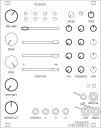
\includegraphics[width=0.7\textwidth]{patch-clean-slate.pdf}\vspace{5mm}\end{center}

Pass through clean unaffected signal.

\end{minipage}\begin{minipage}{0.05\textwidth}\phantom{ }\end{minipage}\begin{minipage}[t]{0.45\textwidth}\setlength{\parskip}{6pt}

\subsection{Saturation}

\vspace{5mm}\begin{center}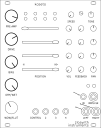
\includegraphics[width=0.7\textwidth]{patch-saturation.pdf}\vspace{5mm}\end{center}

Saturated signal without any delay or effects. Play with the PRE-AMP, DRIVE,
BIAS and DRY/WET controls to achieve the desired sound. Try different input
sources.

Stronger PRE-AMP usually produces more pronounced saturation, but be careful
not to let it clip.

\end{minipage}

\newpage
\noindent\begin{minipage}[t]{0.45\textwidth}\vspace{1cm}\setlength{\parskip}{6pt}

\subsection{Ping pong delay}

\vspace{5mm}\begin{center}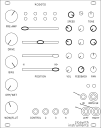
\includegraphics[width=0.7\textwidth]{patch-ping-pong-echo.pdf}\vspace{5mm}\end{center}

The two top-most heads play the incoming signal with a delay set via POSITION.
They are placed left and right using PAN.
Note that VOL of both of these heads is reduced to avoid compression or
clipping.

The last head is enabled with FEEDBACK, feeding the signal back to the beginning
to sustain the echo.

\end{minipage}\begin{minipage}{0.05\textwidth}\phantom{ }\end{minipage}\begin{minipage}[t]{0.45\textwidth}\vspace{1cm}\setlength{\parskip}{6pt}

\subsection{Haas effect and reverb}

\vspace{5mm}\begin{center}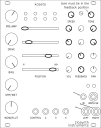
\includegraphics[width=0.7\textwidth]{patch-almost-reverb.pdf}\vspace{5mm}\end{center}

The first two heads, playing left and right with a short delay in between, model
a Haas effect. This effect makes the mono input sound wide in the stereo output.

The two other heads are enabled with FEEDBACK. The feedback signal is filtered
with a low-pass filter configured using TONE. This produces a very simple
reverb. If the output sound grows into a loud feedback loop, set TONE or
FEEDBACK a little lower.

\end{minipage}

% Start of the last page
\newpage

\noindent
\begin{minipage}[t]{0.3\textwidth}
\setlength{\parskip}{6pt}
\section{Acknowledgments}

Kudos to all the eurorack, DSP, and embedded programming communities online.
Here are some of the valuable resources that helped shape this module:

Jatin Chowdhury's white papers
\textit{Real-time physical modelling for analog tape machines\footnote{
  \url{https://ccrma.stanford.edu/~jatin/420/tape/TapeModel_DAFx.pdf}
}}
and
\textit{Complex nonlinearities for audio signal processing\footnote{
  \url{https://ccrma.stanford.edu/~jatin/papers/Complex_NLs.pdf}
}},
and his open-source plugin
\textit{ChowTape\footnote{
  \url{https://github.com/jatinchowdhury18/AnalogTapeModel/}
}}. These materials served as the base for Kaseta's hysteresis model.

Nigel Redmon's blog
\textit{EarLevel Engineering\footnote{
  \url{https://www.earlevel.com/}
}}
and specifically his series about oversampling%
\footnote{\url{https://www.earlevel.com/main/category/digital-audio/sample-rate-conversion/}}.

mhampton's implementation%
\footnote{\url{https://github.com/mhampton/ZetaCarinaeModules}}
of the Ornstein-Uhlenbeck algorithm, which was used as part of the wow effect.

And last but not least, Hainbach%
\footnote{\url{https://www.youtube.com/@Hainbach}}
and his contaigious enthusiasm about tape machines. Which sparked my initial
ideas to create this module.

\vspace{2.5cm}

\end{minipage}%
\begin{minipage}{0.05\textwidth}
\phantom{ }
\end{minipage}%
% Center column
\begin{minipage}[t]{0.3\textwidth}
\section{Changelog}

\begin{tabular}{@{}rl@{}}
  v1.0 & The status LED blinks once
\end{tabular}

\end{minipage}
\begin{minipage}{0.05\textwidth}
\phantom{ }
\end{minipage}%
% Right column
\begin{minipage}[t]{0.3\textwidth}
\setlength{\parskip}{6pt}
\section{Questions?}

You can find more information about the module on
\url{https://zlosynth.com/kaseta}.

\vspace{3mm}

\begin{center}
petr@zlosynth.com
\end{center}
\end{minipage}

\end{document}
